\vspace{-1em}
\section{实验}
\label{sec:exp}
\vspace{-1em}

\subsubsection{训练设置。}

我们使用 AdamW 优化器训练模型 1M 次迭代，批大小为 1；其中仅将 Memory Attention、Mask Decoder 和 Feature Merger 设为可训练，学习率分别为 5e-6、5e-6 和 1e-5。所有损失系数以及设为 8 的记忆帧数均遵循原始 SAM2 配置。


\vspace{-1em}
\subsubsection{数据集。}



\begin{table}[t]
\centering
\small
\setlength{\tabcolsep}{2mm}
\vspace{-3mm}
\caption{\textbf{用于训练的数据集。}
仅当真值几何可用时，我们才应用 FOV 感知采样。}
\label{tab:datasets}
\vspace{-3mm}
    \begin{tabular}{lccc}
    \toprule
    & ScanNet++~\cite{yeshwanth2023scannet++} & ASE~\cite{avetisyan2024scenescript} & MOSE~\cite{MOSE} \\
    \midrule
    真实                        & \ding{51} & \ding{55}          & \ding{51} \\
    动态                     & \ding{55}          & \ding{55}          & \ding{51} \\
    FOV 采样概率           & 0.8        & 0.8        & 0.0 \\
    \#场景/视频           & 855        & 2612        & 1453 \\
    \bottomrule
    \end{tabular}
% }
\vspace{-3mm}
\end{table}


直观地说，为了使模型具备在整个场景中一致分割对象的能力，需要在基于 3D 的数据集上训练；这些数据集记录了覆盖多样相机视角的长视频序列，并提供相应分割掩码和 RGB 帧。然而，此类 3D 数据集中的 2D 掩码通常由点云分割投影而来，可能会因点云稀疏性和投影误差而退化。

为缓解 3D 数据集中常见的不完美 2D 掩码标注问题，我们混合使用合成、真实和视频分割数据集进行训练。具体而言，Aria Synthetic Dataset (ASE)~\cite{avetisyan2024scenescript} 提供干净的几何监督，ScanNet++~\cite{yeshwanth2023scannet++} 提供真实室内 3D 一致性，MOSE\cite{MOSE} 保留原始时间一致掩码。这一组合实现了空间和时间学习之间的平衡。需要注意的是，为与 \cref{subsec:sampling} 中的采样策略保持一致，由于 MOSE 不提供相机位姿或深度图，我们在 MOSE 上采用连续采样。
对于包含标定几何的 ASE 和 ScanNet++，我们采用混合策略：以 0.2 的概率进行连续采样，以 0.8 的概率进行 FOV 感知采样。
FOV 阈值 $\tau$ 设为 0.25。为应用我们的采样策略，我们首先在 ScanNet++ 和 MOSE 的每个场景上运行 MUSt3R 推理，并存储得到的特征。这些预计算特征随后在训练期间用于启用 FOV 感知采样。
对于连续采样的 batch，MUSt3R 会即时执行。  



\vspace{-0.5em}
\subsection{2D 评估。}
\vspace{-0.5em}

为展示模型能力，我们评估其在挑战性相机运动下的 2D 对象跟踪性能。
具体而言，我们关注相机发生显著平移和旋转、对象可能消失后重现的场景。
LVOS~\cite{hong2023lvos}、VOST~\cite{tokmakov2023vost}、DAVIS~\cite{perazzi2017davis} 和 YTOS~\cite{xu2018youtube} 等传统 VOS 基准主要假设相机相对固定、场景环境稳定，因此不足以测试大幅视角变化下的鲁棒性。

为解决这一限制，我们使用基于 3D 的数据集 ScanNet++~\cite{yeshwanth2023scannet++} 和 Replica~\cite{replica19arxiv}；由于 3D 重建需求，它们天然提供了丰富的相机轨迹变化。
其宽基线视角适合评估剧烈位姿变化下的一致性。
对于两个数据集中的每个场景，我们使用真值相机位姿将 3D 实例掩码投影到 2D 帧。
随后选择可见掩码面积最大的帧作为条件帧，并从该参考帧执行正向和反向跟踪。

\vspace{-1em}
\subsubsection{比较方法。}
作为比较，我们使用 SAM2 作为最先进的 VOS 基线。
我们还纳入 SAM2Long~\cite{ding2024sam2long} 和 DAM4SAM~\cite{videnovic2025distractor}，它们通过改进 SAM2 的记忆选择来实现更鲁棒的跟踪。需要注意的是，除非另有说明，我们的方法 \textbf{3AM} 在所有报告结果中均使用原始 SAM2 的朴素记忆机制。

\vspace{-1em}
\subsubsection{指标。}
我们使用三个互补指标评估跟踪质量。
\textbf{IoU} 在所有帧上计算，包括对象不存在的帧，反映整体稳定性。
\textbf{Tracking Recall} 仅在目标对象存在的帧上衡量准确性。
\textbf{Accuracy} 进一步限制在预测与真值具有非零重叠的可见帧上，刻画成功定位条件下的准确性。
这些指标共同评估对对象消失的鲁棒性以及跟踪成功时的准确性。

\vspace{-1em}
\subsubsection{ScanNet++.}

\begin{table*}[t]
\centering
\small
\vspace{-3mm}
\caption{\textbf{ScanNet++ \cite{yeshwanth2023scannet++} 和 VOS 数据集上的视频对象分割结果。}
Tracking Recall 在对象存在的帧上计算。
Accuracy 在存在真值对象且预测与 GT 的 IoU $\neq 0$ 的帧上计算。}
\label{tab:scannetpp-2d}
  \vspace{-3mm}
\resizebox{\textwidth}{!}{
\begin{tabular}{lcccccccccccc}
\toprule
\multirow{2}{*}{Method} &
\multirow{2}{*}{FPS} &
Mem &
\multicolumn{3}{c}{ScanNet++ Whole Set} &
\multicolumn{3}{c}{ScanNet++ Selected Subset} & $\text{DAVIS}_{17}$ & LaSOT & $\text{LaSOT}_{\text{ext}}$ & DiDi \\
\cmidrule(lr){3-3}\cmidrule(lr){4-6} \cmidrule(lr){7-9} \cmidrule(lr){10-10} \cmidrule(lr){11-11} \cmidrule(lr){12-12} \cmidrule(lr){13-13}
& & G & IoU $\uparrow$ & Tracking Recall $\uparrow$ & Accuracy $\uparrow$ & IoU $\uparrow$ & {Tracking Recall} $\uparrow$ & Accuracy $\uparrow$ & J\&F $\uparrow$  & AUC $\uparrow$  & AUC $\uparrow$  & Accuracy $\uparrow$  \\
\midrule
SAM2~\cite{ravi2024sam2}  & 14.4 & 3.6 & 0.4392 & 0.0235 & 0.0831 & 0.3397 & 0.0179 & 0.0395 & 89.0 & 70.0 & 56.9 & 0.720 \\
SAM2Long~\cite{ding2024sam2long} & 7.1 & 6.8 & \cellcolor{orange!25}0.8233 & \cellcolor{yellow!25}0.4166 & \cellcolor{orange!25}0.6855 & \cellcolor{yellow!25}0.7474 & \cellcolor{yellow!25}0.4133 &  \cellcolor{yellow!25}0.6382 & 88.3 & 73.9 & - & 0.719 \\
DAM4SAM~\cite{videnovic2025distractor} & 12.3 & 3.5 & \cellcolor{yellow!25}0.8205 & \cellcolor{orange!25}0.4193 & \cellcolor{yellow!25}0.6783 & \cellcolor{orange!25}0.7648 & \cellcolor{orange!25}0.4356 & \cellcolor{orange!25}0.6650 & 86.6 & 75.1 & 60.9 & 0.727\\
3AM & 6.3 & 3.6 & \cellcolor{red!25}0.8898 & \cellcolor{red!25}0.5630 & \cellcolor{red!25}0.7155 & \cellcolor{red!25}0.9061 & \cellcolor{red!25}0.7168 & \cellcolor{red!25}0.7737 & 89.0 & 70.0 & 56.9 & 0.720 \\
\bottomrule
\end{tabular}
}
\vspace{-3mm}
\end{table*}

\begin{figure*}[t]
    \centering
    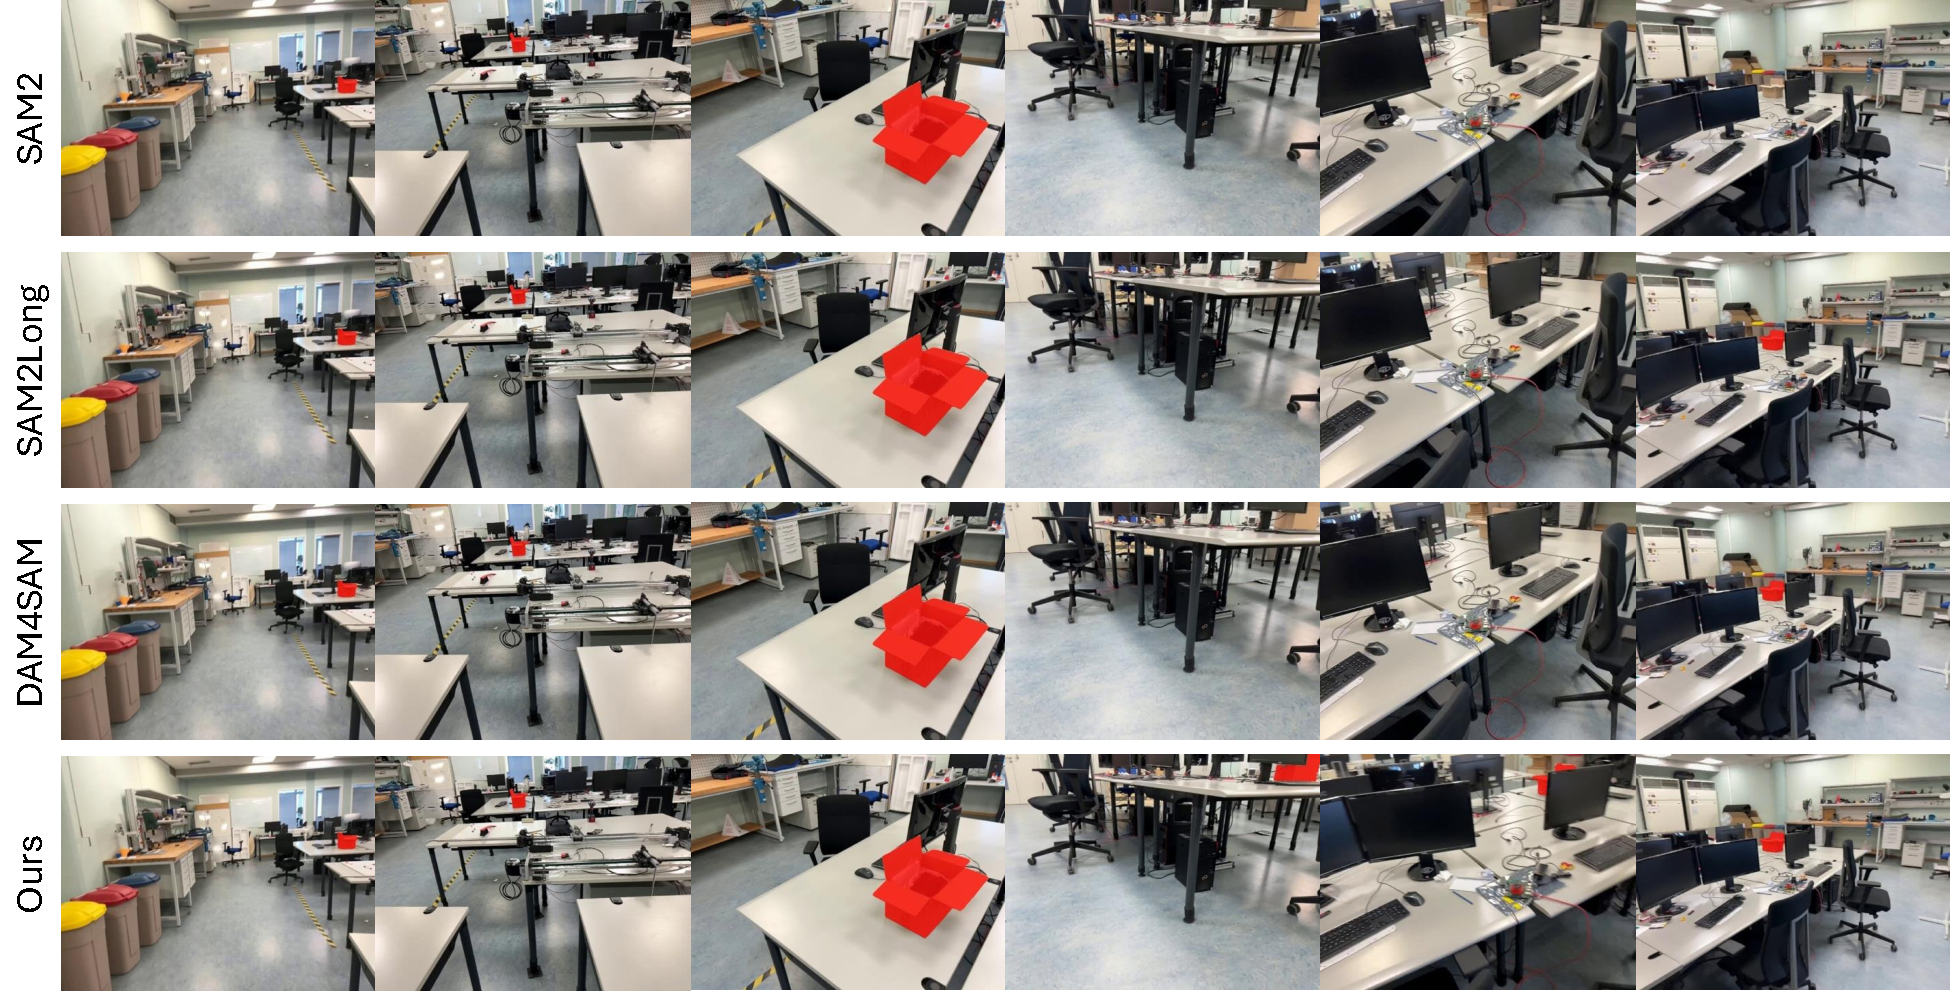
\includegraphics[width=1.0\textwidth]{figs/vis_comp.pdf}
    \vspace{-6mm}
    \caption{
    \textbf{VOS 方法的视觉比较。} 最左侧帧作为条件帧，并提供参考掩码。
    }
    \label{fig:vis_comp}
\end{figure*}

结果如 \cref{tab:scannetpp-2d} 所示，可视化见 \cref{fig:vis_comp}。
在 ScanNet++ 数据集上，我们进一步在专门构造以突出对象重现的 \emph{Selected Subset} 上评估性能。
对于每条对象轨迹，我们统计非连续可见片段数量，其中一个片段定义为长度 $\ell$ 超过最小阈值 $\ell_{\min}$ 的任意连续可见帧区间。
频繁重现的对象通常伴随大幅视角变化，因为每次消失—重现循环往往对应于从显著不同的角度或位置观察对象。
因此，该子集能集中评估剧烈位姿变化下的鲁棒性。

3AM 在 \emph{Whole Set}（IoU 0.8898，Recall 和 Accuracy 最高）和更具挑战性的 \emph{Selected Subset}（IoU 0.9061、Recall 0.7168、Accuracy 0.7737）上均取得最佳性能，突显出即便对象在视角和空间配置大幅变化后重现，它仍能保持对象身份。借助简单回退机制，它在传统 VOS 基准~\cite{perazzi2017davis, fan2019lasot, videnovic2025distractor} 上也保持了有竞争力的结果，如 \cref{tab:scannetpp-2d} 所示。

\vspace{-1em}
\subsubsection{与 SegMASt3R 的两视图匹配比较。}
我们进一步在 \cref{tab:two_view_comparison} 中将 3AM 与 SegMASt3R~\cite{Jayanti2025SegMASt3R} 比较。SegMASt3R 是一种基于 MASt3R 的两视图匹配方法，可在大幅视角变化下关联两张图像之间的分割掩码。SegMASt3R 不能直接被提示，也不原生支持 $>2$ 的多视图跟踪。尽管如此，我们仍将其作为强两视图基线，并采用如下协议：使用真值初始掩码作为源帧候选；对于每个后续帧，独立执行其与源帧之间的两视图掩码匹配。为公平比较两种方法，使用 3AM 跟踪时，我们不使用源帧之外的任何记忆。

在该协议下，3AM 的 \textbf{IoU}、\textbf{Tracking Recall} 和 \textbf{Accuracy} 分别达到 $0.8915$、$0.5115$ 和 $0.6405$，而 SegMASt3R 分别为 $0.6800$、$0.3628$ 和 $0.4053$。这些结果表明，3AM 不仅功能更强，即使限制在两视图匹配设置下也优于 SegMASt3R。

\begin{table}[t]
\centering
\setlength{\tabcolsep}{2mm}
\vspace{-3mm}
\begin{minipage}{0.48\textwidth}
\centering
\caption{{3AM 与 SegMASt3R 在 ScanNet++ Whole Set 上的两视图匹配定量比较。}}
\label{tab:two_view_comparison}
\vspace{-3mm}
\resizebox{\textwidth}{!}{
\begin{tabular}{lccc}
\toprule
方法 & IoU $\uparrow$ & {Tracking Recall} $\uparrow$ & Accuracy $\uparrow$\\
\midrule
SegMASt3R~\cite{Jayanti2025SegMASt3R} & 0.6800 & 0.3628 & 0.4053 \\
\rowcolor{black!10}
3AM (Ours) & \textbf{0.8915} & \textbf{0.5115} & \textbf{0.6405} \\
\bottomrule
\end{tabular}
}
\end{minipage}
\begin{minipage}{0.48\textwidth}

\centering
\caption{{Replica\cite{replica19arxiv} 数据集上的视频对象分割结果。}}
\label{tab:replica-3d}
\vspace{-3mm}
\resizebox{\textwidth}{!}{
\begin{tabular}{lccc}
\toprule
方法 & IoU $\uparrow$ & Tracking Recall $\uparrow$ & Accuracy $\uparrow$ \\
\midrule
SAM2~\cite{ravi2024sam2} & 0.4424 & 0.1432 & 0.2188 \\
SAM2Long~\cite{ding2024sam2long} & \cellcolor{yellow!25}0.7691 & \cellcolor{orange!25}0.5195 & \cellcolor{orange!25}0.6273 \\
DAM4SAM~\cite{videnovic2025distractor} & \cellcolor{orange!25}0.7744 & \cellcolor{yellow!25}0.5135 & \cellcolor{yellow!25}0.6124 \\
3AM (Ours) & \cellcolor{red!25}0.8119 & \cellcolor{red!25}0.6381 &  \cellcolor{red!25}0.6793 \\
\bottomrule
\end{tabular}
}
\end{minipage}

\vspace{-3mm}
\end{table}


\vspace{-1em}
\subsubsection{Replica。}

在 Replica 数据集上，3AM 在所有指标上均取得最佳性能（\cref{tab:replica-3d}），IoU 达到 0.8119，超过 SAM2（0.4424）、SAM2Long（0.7691）和 DAM4SAM（0.7744）。它还取得最高 Tracking Recall（0.6381）和 Accuracy（0.6793），展示了在 Replica 特有的大幅视角变化下的鲁棒跟踪能力。

这些结果表明，尽管 3AM 不依赖先前方法使用的显式记忆选择机制，它仍能持续超越以往方法，并且在对象重现和大幅视角变化场景中特别有效。受篇幅限制，更多可视化结果见补充材料。


\vspace{-0.5em}
\subsection{3D 评估}
\vspace{-0.5em}

接下来，我们在一个 3D 任务上评估方法。
我们采用 ScanNet200 的类别无关 3D 实例分割设置，因为它直接反映模型在 3D 场景中生成对象一致预测的能力。
以往方法通常需要显式 3D 融合\cite{xu2024esam} 或合并\cite{yang2023sam3d}，无论提议来自 2D 掩码\cite{jung2025details} 还是 3D 检测器\cite{boudjoghra2025openyolo, nguyen2024open3dis}。
我们的目标是证明这种额外的 3D 空间合并并非必要：如果 2D 跟踪在跨视角下具有几何一致性，那么只需将跟踪得到的 2D 掩码投影到 3D，即可获得可靠的 3D 实例。

具体而言，我们遵循以往方法\cite{zhao2025sam2object}，在基于步长采样选出的关键帧上使用 SAM2 生成 2D 提议。
随后使用 3AM 传播这些提议；其增强的跨视角一致性使模型能够在多个相机视角中稳定识别对象。
我们使用 IoU 和掩码间精度在时间上关联提议，并将得到的 2D 轨迹投影到 3D。
相比之下，以往基于 SAM2 的方法\cite{zhao2025sam2object} 高度依赖 3D 合并，因为其跟踪在大幅视角变化下常会漂移或失败。
更多实现细节见补充材料。

如 Table~\ref{tab:scannet200-class-agnostic} 所示，3AM 在在线方法中取得最高性能，AP 为 47.3，AP$_{50}$ 和 AP$_{25}$ 也表现强劲（59.7 和 75.3）。
这些结果突显了本文的一个核心发现：无需大量 3D 监督，鲁棒的 3D 实例分割也可以从几何感知跟踪中涌现。



\begin{table}[t]
\centering
\small
\setlength{\tabcolsep}{2mm}
\vspace{-3mm}
\caption{\textbf{不同方法在 ScanNet200 数据集上的类别无关 3D 实例分割结果。}}
\label{tab:scannet200-class-agnostic}
\vspace{-3mm}
\begin{tabular}{lccccc}
\toprule
方法 & 类型 & 3D GT & AP $\uparrow$ & AP$_{50}$ $\uparrow$ & AP$_{25}$ $\uparrow$ \\
\midrule
SAMPro3D~\cite{xu2025sampro3d} & 离线 & 是 & 18.0 & 32.8 & 56.1 \\
Open3DIS~\cite{nguyen2024open3dis} & 离线 & 是 & \cellcolor{yellow!25}34.6 & 43.1 & 48.5 \\
SAI3D~\cite{yin2024sai3d} & 离线 & 是 & 28.2 & 47.2 & 67.9 \\
SAM2Object~\cite{zhao2025sam2object} & 离线 & 是 & 34.0 & \cellcolor{yellow!25}52.7 & \cellcolor{yellow!25}70.3 \\
\midrule
SAM3D~\cite{yang2023sam3d} & 在线 & 是 & 20.2 & 35.7 & 55.5 \\
ESAM~\cite{xu2024esam} & 在线 & 是 & \cellcolor{orange!25}42.2 & \cellcolor{red!25}63.7 & \cellcolor{red!25}79.6 \\
\midrule
3AM (Ours) & 在线 & 否 & \cellcolor{red!25}47.3 & \cellcolor{orange!25}59.7 & \cellcolor{orange!25}75.3 \\
\bottomrule
\end{tabular}
% }
\vspace{-3mm}
\end{table}


\vspace{-0.5em}
\subsection{消融研究}
\vspace{-0.5em}

\subsubsection{组件分析。}
我们在 \cref{tab:component-eval} 中针对 Feature Source、Feature Merger Architecture 和 Sampling Strategy 进行消融研究。
我们在相同训练协议下评估仅使用 MUSt3R 或 SAM2 特征的变体，以证明两类特征都是必要的。MUSt3R 提供几何锚定，而 SAM2 捕获外观对应。没有 MUSt3R 时，仅依赖 SAM2 的外观匹配会引入歧义并导致性能下降。需要注意的是，SAM2 在微调后表现更差。我们将这一退化归因于缺少来自 MUSt3R 的锚定信息，导致记忆注意力因缺乏区分不同对象的参考线索而被错误训练。
关于采样策略，朴素应用随机采样的性能差于连续采样。当两个视角中都存在有效掩码时，强制关联空间差异很大的区域会引入歧义并导致收敛更慢。

\begin{table*}[t]
\centering
\setlength{\tabcolsep}{2mm}
\caption{\textbf{ScanNet++ selected subset 上的组件分析。}}
\label{tab:component-eval}
\vspace{-3mm}
\resizebox{\textwidth}{!}{%
\begin{tabular}{cccccc}
\toprule
Feature Source & Feature Merger & Sampling Strategy & IoU & Tracking Recall & Accuracy \\
\midrule
SAM2 \& MUSt3R & Addition \& Convolution & FoV Sampling & 0.8771 & 0.6481 & 0.7149\\
SAM2 \& MUSt3R & Concatentation \& Attention & FoV Sampling & 0.8831 & 0.6744 & 0.7462\\
SAM2 \& MUSt3R & Hierarchical Cross Attention (Final) & Continuous Sampling & 0.7925 & 0.6518 & 0.7513\\
SAM2 \& MUSt3R & Hierarchical Cross Attention (Final) & Random Sampling & 0.7363 & 0.5371 & 0.6311 \\
MUSt3R  & - & FoV Sampling & 0.8461 & 0.5471 & 0.4129 \\
SAM2 & - & FoV Sampling & 0.6628 & 0.0038 & 0.0276 \\
SAM2 \& MUSt3R & Hierarchical Cross Attention (Final) & FoV Sampling & 0.9061 & 0.7168 & 0.7737\\
\bottomrule
\end{tabular}
}
\end{table*}

\vspace{-1em}
\subsubsection{记忆选择。}
\label{subsubsec-memory-select}

\begin{table}[t]
\centering
\small
\setlength{\tabcolsep}{2mm}
\vspace{-3mm}

\begin{minipage}{0.48\textwidth}
\caption{ScanNet++ Whole Set 上不同记忆选择方法的比较。}
\label{tab:memory-selection}
\vspace{-3mm}
\resizebox{\textwidth}{!}{
\begin{tabular}{lccc}
\toprule
方法 & IoU $\uparrow$ & Tracking Recall $\uparrow$ & Accuracy $\uparrow$ \\
\midrule
3AM & \cellcolor{yellow!25}0.8898 & \cellcolor{yellow!25}0.5630 & \cellcolor{yellow!25}0.7155 \\
DAM4SAM-3AM~\cite{videnovic2025distractor} & \cellcolor{orange!25}0.8941 & \cellcolor{orange!25}0.5471 &  \cellcolor{orange!25}0.7204 \\
SAM2Long-3AM~\cite{ding2024sam2long} & \cellcolor{red!25}0.9004 & \cellcolor{red!25}0.5498 & \cellcolor{red!25}0.7361 \\
\bottomrule
\end{tabular}
}
\end{minipage}
\begin{minipage}{0.48\textwidth}
\caption{不同 3D 重建骨干网络的比较。}
\label{tab:3D_backbone}
\resizebox{\textwidth}{!}{
\begin{tabular}{lccc}
\toprule
\textbf{模型} & \textbf{在线} & \textbf{帧数} & \textbf{ScanNet++ Selected Subset Tracking Recall} \\
\midrule
VGGT & $\times$ & $\sim$200       & --      \\
$\pi^3$ & $\times$ & $\sim$300    & --      \\
CUT3R & \checkmark & $>10{,}000$  &  0.2751 \\
\rowcolor{black!10}
MUSt3R & \checkmark & $>10{,}000$  &  \textbf{0.7168}  \\
\bottomrule
\end{tabular}
}
\end{minipage}
\vspace{-3mm}
\end{table}

我们进一步通过将 3AM 与现有 SAM2 记忆选择策略结合来分析记忆选择的作用。
Table~\ref{tab:memory-selection} 报告了 ScanNet++ Whole Set 上的结果。
使用原始 SAM2 记忆选择机制的 3AM 已经取得强劲性能，IoU 为 0.8898。
当我们引入 DAM4SAM~\cite{videnovic2025distractor} 或 SAM2Long~\cite{ding2024sam2long} 等替代记忆选择策略时，观察到适度提升：DAM4SAM-3AM 将 Accuracy 略微提升到 0.7204，而 SAM2Long-3AM 取得最高 IoU（0.9004）和 Accuracy（0.7361）。
这些结果表明，即使不依赖专门的记忆选择策略，3AM 已能提供强大且稳定的性能。
尽管 SAM2Long 或 DAM4SAM 等替代策略可带来少量额外增益，但与 3AM 本身带来的提升相比，其影响相对有限。
我们认为，为 3AM 专门设计记忆选择机制是未来一个有趣方向。

\vspace{-1em}
\subsubsection{3D 基础模型。}
\label{subsubsec-3d-models}

\begin{figure}[t]
    \centering
    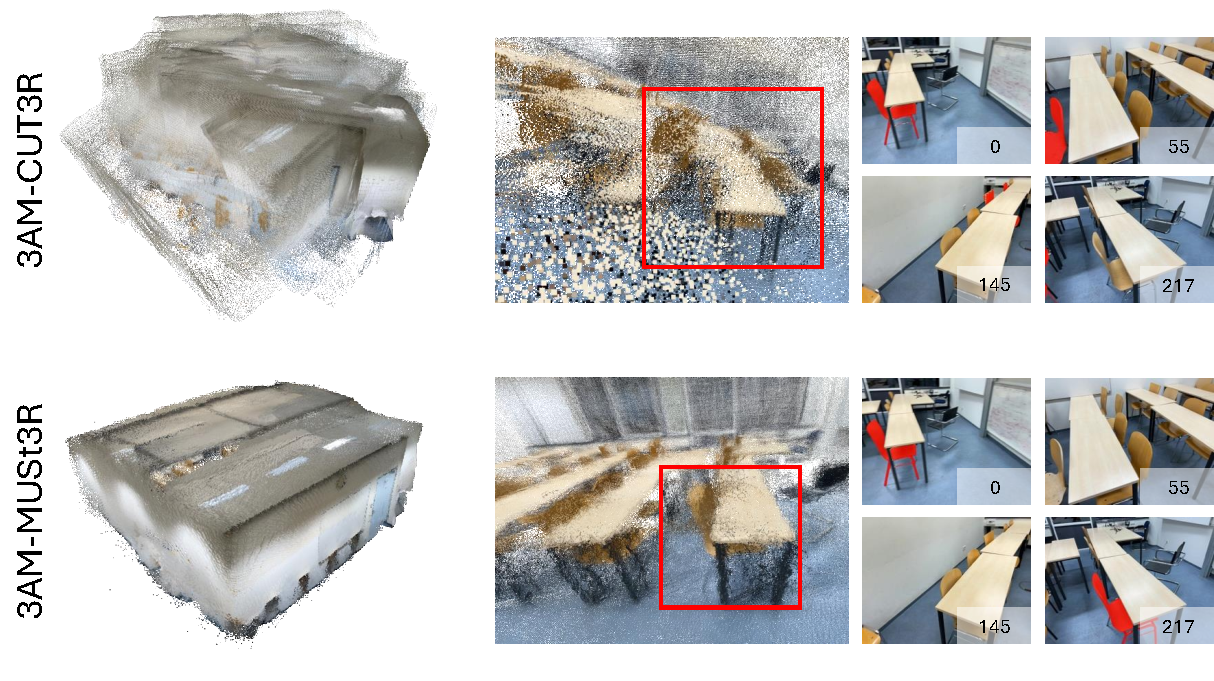
\includegraphics[width=1.0\linewidth]{figs/vis_cut3r.pdf}
    \vspace{-6mm}
    \caption{
    \textbf{不同 3D 重建骨干网络的视觉比较。}（\emph{上}）CUT3R 的重建缺乏稳定对象对齐；同一张桌子出现在不一致的 3D 位置。这种几何不稳定性削弱了特征区分性，使可靠跟踪变得困难。（\emph{下}）相比之下，MUSt3R 在跨视角下提供连贯且稳定的对象对齐，生成能够保持对象身份并支持鲁棒跟踪的特征
    }
    \label{fig:comp_3r}
\end{figure}

我们在 Table~\ref{tab:3D_backbone} 中比较 3D 基础模型。VGGT 和 $\pi^3$ 在帧 batch 上离线运行，不适合在线跟踪。CUT3R 支持在线运行，但如 \cref{fig:comp_3r} 所示，其实例级对齐有限，这也反映在它在 ScanNet++ Selected Subset 上仅有 0.2751 的 Tracking Recall。MUSt3R 完全在线，并在跨视角对象对齐方面显著更强。这种对齐至关重要：一致的 3D 对齐支持稳定的 2D 跨视角对应，使模型无需显式 3D 合并即可可靠传播掩码。


